\documentclass[conference]{IEEEtran}
\IEEEoverridecommandlockouts
% The preceding line is only needed to identify funding in the first footnote. If that is unneeded, please comment it out.
\usepackage{cite}
\usepackage{amsmath,amssymb,amsfonts}
\usepackage{algorithmic}
\usepackage{graphicx}
\usepackage{textcomp}
\usepackage{xcolor}
\usepackage{todonotes}

\def\BibTeX{{\rm B\kern-.05em{\sc i\kern-.025em b}\kern-.08em
    T\kern-.1667em\lower.7ex\hbox{E}\kern-.125emX}}
\begin{document}

\title{Sparse State Estimation under Sensor Corruption \\

}

\author{\IEEEauthorblockN{Gokul Rajaraman}
\IEEEauthorblockA{\textit{Dept. of Mechanical Engg.} \\
\textit{IIT Bombay}\\
Mumbai, India \\
22b4517@iitb.ac.in}

\and
\IEEEauthorblockN{Rohan Badgujar}
\IEEEauthorblockA{\textit{Dept. of Mechanical Engg.} \\
\textit{IIT Bombay}\\
Mumbai, India \\
22b2196@iitb.ac.in}

}

\maketitle

\begin{abstract}
This project studies robust state estimation for dynamical systems in the presence of sparse sensor corruption. In many cyber-physical systems, sensor measurements may be affected by noise, faults, or adversarial attacks, causing conventional least-squares estimators to produce inaccurate state estimates. To address this problem, we formulate a sparse recovery framework that jointly estimates the system state and sparse sensor corruption. For linear dynamical systems, the estimation problem is posed as an $L_1$-regularized batch optimization problem, which serves as a computationally tractable relaxation of the ideal sparse $L_0$ formulation. The framework is then extended to a nonlinear benchmark based on a coupled damped pendulum network using sequential convex programming and nonlinear optimization methods. Numerical experiments are performed to study the effect of regularization, process noise, and measurement noise on corruption recovery performance. The results show that moderate regularization achieves the best tradeoff between sparsity and estimation accuracy, while increasing noise levels degrade recovery quality. 
\end{abstract}

\section{Introduction}
Modern estimation and control systems increasingly rely on sensor data to infer the internal state of a dynamical system. In practice, however, sensor measurements are rarely perfect. They may be affected by random noise, modeling mismatch, or persistent corruption caused by faulty hardware or adversarial interference. When even a small subset of sensors is corrupted, standard least-squares estimation can become unreliable because the corrupted readings can bias the recovered state significantly. This makes robust state estimation an important problem in cyber-physical systems, robotics, and networked control. The central idea in this project is to jointly estimate the system state and identify sparse sensor corruption by exploiting the sparsity under the assumption that only a few sensors are affected at any given time. 

In this work, we study sparse state estimation under sensor corruption for both linear and nonlinear dynamical systems. For the linear case, we model the system in discrete time with process noise, measurement noise, and sparse additive corruption on the outputs. The sparse corruption is recovered using an \(L_1\)-regularized batch optimization framework, which serves as a convex relaxation of the ideal but combinatorial \(L_0\) formulation. We then extend the same estimation idea to a nonlinear benchmark based on a coupled damped pendulum network, where the dynamics are handled using sequential convex programming and nonlinear optimization solvers such as OSQP\cite{osqp} and IPOPT \cite{ref:waechter-biegler-ipopt-2006}. Across both settings, the results show that moderate regularization provides the best balance between data fit and sparsity, while increasing process noise or measurement noise makes corruption recovery more difficult.

We have used several references for this work. The main works that introduce the sparse sensor bias include \cite{sandberg2022secure,mishra2017secure}. Other works, such as \cite{das2025algorithmic}, provide algorithmic recipes to detect false data injection attacks in linear systems. Several survey papers, such as \cite{ding2018survey,giraldo2018survey,mitchell2014survey,he2016cyber}, are among our references.
\section{Problem Statement}

The objective of this project is to perform robust state estimation in the presence of sparse sensor corruption. In practical dynamical systems, sensor measurements are often affected not only by random process and measurement noise, but also by persistent faults or adversarial corruption in a small subset of sensors. Such corruption can significantly bias the estimated system state if conventional least-squares estimation methods are used. Therefore, the estimator must simultaneously recover the system state and identify the corrupted sensor channels.

For the linear case, the discrete-time system is modeled as
\begin{equation}
x_{k+1} = Ax_k + Bu_k + w_k
\end{equation}

\begin{equation}
y_k = Cx_k + e_k + v_k
\end{equation}

where $x_k \in \mathbb{R}^n$ represents the system state, $u_k \in \mathbb{R}^m$ is the known control input, $w_k$ and $v_k$ denote process and measurement noise respectively, and $e_k \in \mathbb{R}^p$ represents sparse sensor corruption. The key assumption is that only a small number of sensors are corrupted at any given time, i.e.,
\begin{equation}
\|e_k\|_0 \leq s \ll p
\end{equation}

The primary goal is to jointly estimate the state trajectory $\{x_k\}$ and identify the sparse corruption vector $\{e_k\}$ from noisy and partially corrupted measurements.

An ideal sparse recovery formulation uses an $L_0$ sparsity constraint, but solving such a problem requires combinatorial search over sensor subsets and becomes computationally intractable for larger systems. To overcome this difficulty, the project employs an $L_1$-regularized convex relaxation approach, which promotes sparsity while remaining efficiently solvable using convex optimization techniques.

In addition to the linear system, the project also investigates a nonlinear benchmark based on a coupled damped pendulum network. The nonlinear model introduces additional challenges due to nonlinear restoring forces and coupling between neighboring pendulums. Sparse state estimation for this case is solved using sequential convex programming and nonlinear optimization methods such as OSQP and IPOPT.

Overall, the problem addressed in this work is the robust recovery of hidden system states under sparse sensor corruption, while analyzing the influence of regularization, process noise, and measurement noise on estimation performance.

\section{System Model}

\subsection{Linear Dynamical System}

The linear system considered in this project is modeled in discrete time as
\begin{equation}
x_{k+1} = Ax_k + Bu_k + w_k,
\end{equation}
\begin{equation}
y_k = Cx_k + e_k + v_k,
\end{equation}
where $x_k \in \mathbb{R}^n$ denotes the system state, $u_k \in \mathbb{R}^m$ is the known control input, $y_k \in \mathbb{R}^p$ is the measurement vector, $w_k$ is the process noise, $v_k$ is the measurement noise, and $e_k$ represents sparse sensor corruption. The process and measurement noises are assumed to be zero-mean Gaussian, consistent with the simulation setup used in the experiments. The central estimation objective is to recover both the state trajectory $\{x_k\}$ and the sparse corruption sequence $\{e_k\}$ from partially observed and corrupted measurements. \cite{linearModel}

In the linear experiments, the system is chosen to be partially observed, with only a subset of the states directly measured. The observation matrix is structured so that the remaining states must be inferred through the coupling induced by the dynamics matrix. The dynamics matrix is selected to be stable, which ensures that the open-loop trajectory remains bounded during simulation. The control input is included in the forward simulation, while the estimation stage focuses on recovering the state and corruption from the measured outputs. \cite{linearModel}

\subsection{Sparse Sensor Corruption Model}

The corruption term $e_k$ is assumed to be sparse in the sensor dimension, meaning that only a small number of sensors are corrupted at any given time. In the linear experiments, the corrupted sensor indices are fixed over time, so the corruption behaves like a persistent sensor bias rather than a transient spike. This model is appropriate for representing faulty sensors or adversarial interference that affects only a limited subset of outputs. \cite{linearModel}

\subsection{Nonlinear Benchmark System}

To extend the same estimation framework to a nonlinear setting, a coupled damped pendulum network is used as a benchmark system. The state is defined as
\begin{equation}
x_k =
\begin{bmatrix}
\theta_k \\
\omega_k
\end{bmatrix}
\in \mathbb{R}^{2N},
\end{equation}
where $\theta_k \in \mathbb{R}^{N}$ contains the pendulum angles and $\omega_k \in \mathbb{R}^{N}$ contains the angular velocities. The output equation retains the same sparse corruption structure,
\begin{equation}
y_k = Cx_k + e_k + v_k,
\end{equation}
but the state evolution is now governed by nonlinear coupled dynamics. \cite{nonlinearModel}

The discrete-time nonlinear dynamics used in the experiments are
\begin{equation}
\theta_{k+1} = \theta_k + dt\,\omega_k,
\end{equation}
\begin{equation}
\omega_{k+1} = \omega_k + dt\left(-a\sin(\theta_k) - d\omega_k + cL\theta_k\right),
\end{equation}
where $a$ controls the restoring torque, $d$ is the damping coefficient, $c$ is the coupling gain, and $L$ is the Laplacian matrix representing nearest-neighbor interactions along the chain. This benchmark is nonlinear, partially observed, and locally coupled, which makes it a suitable test case for robust sparse state estimation. \cite{nonlinearModel}

\subsection{Assumptions}

The overall estimation problem is studied under the following assumptions:
\begin{itemize}
    \item the state dynamics are known up to the simulation model,
    \item only a small subset of sensors is corrupted,
    \item process and measurement noises are additive,
    \item the corruption is sparse in the output dimension,
    \item the nonlinear benchmark is locally coupled through the graph Laplacian.
\end{itemize}


\section{Optimization Formulation}

\subsection{Linear Batch Estimation}

For the linear system, the goal is to jointly estimate the state trajectory and the sparse corruption sequence from corrupted measurements. Using a batch formulation over a finite horizon $N$, the estimation problem can be written as
\begin{equation}
\min_{\{x_k,e_k\}} \sum_{k=0}^{N} \|y_k - Cx_k - e_k\|_2^2
\end{equation}
subject to the dynamics constraint
\begin{equation}
x_{k+1} = Ax_k + Bu_k.
\end{equation}

The corruption term $e_k$ is assumed to be sparse across sensors, so an exact formulation would require a combinatorial search over possible corrupted sensor subsets. This makes the direct $L_0$-based formulation computationally expensive and impractical for moderate to large measurement dimensions. %\cite{fawzi2014secure}

\subsection{Convex $L_1$ Relaxation}

To obtain a tractable estimator, the sparse constraint is relaxed using an $L_1$ penalty. The resulting convex optimization problem is
\begin{equation}
\min_{\{x_k,e_k\}} \sum_{k=0}^{N} \|y_k - Cx_k - e_k\|_2^2 + \lambda \sum_{k=0}^{N}\|e_k\|_1
\end{equation}
subject to
\begin{equation}
x_{k+1} = Ax_k + Bu_k.
\end{equation}

Here, $\lambda$ controls the tradeoff between data fidelity and sparsity. A small value of $\lambda$ may under-penalize corruption and allow noise to leak into the state estimate, while a large value of $\lambda$ may over-penalize the corruption term and suppress valid sparse bias. The experiments in this project show that the best recovery is typically achieved at an intermediate regularization level. %\cite{mishra2017secure}


\subsection{Nonlinear Batch Estimation}

The same sparse recovery idea is extended to the nonlinear benchmark. In that case, the state evolves according to
\begin{equation}
x_{k+1} = f(x_k),
\end{equation}
and the measurements are still corrupted by sparse sensor bias:
\begin{equation}
y_k = h(x_k) + e_k + v_k.
\end{equation}

The nonlinear batch estimation problem becomes
\begin{equation}
\min_{\{x_k,e_k\}} \sum_{k=0}^{N} \|y_k - h(x_k) - e_k\|_2^2 + \lambda \sum_{k=0}^{N}\|e_k\|_1
\end{equation}
subject to
\begin{equation}
x_{k+1} = f(x_k).
\end{equation}

Because the dynamics are nonlinear, the problem is no longer convex. In this project, the nonlinear estimator is handled using two approaches: sequential convex programming with linearization at the current iterate, and direct nonlinear optimization. The first approach yields a sequence of convex subproblems, while the second solves the constrained nonlinear program more directly.

\subsection{Sequential Convex Approximation}

At iteration $i$, the nonlinear dynamics are linearized around the current estimate $\bar{x}_k^{(i)}$:
\begin{equation}
f(x_k) \approx f(\bar{x}_k^{(i)}) + J_f(\bar{x}_k^{(i)})(x_k - \bar{x}_k^{(i)}),
\end{equation}
where $J_f(\bar{x}_k^{(i)})$ is the Jacobian of the dynamics. This produces a convex quadratic subproblem with an $L_1$ penalty on the corruption term. The subproblem is solved repeatedly until convergence. In the implementation, this framework is associated with OSQP-based iterative convex optimization. %\cite{fawzi2014secure}

\subsection{Direct Nonlinear Optimization}

For comparison, the nonlinear estimation problem is also solved directly using an interior-point method. In this formulation, the full nonlinear dynamics are retained and the optimizer searches for the state and corruption sequence that minimize the same regularized objective. This approach is computationally more expensive than sequential convex approximation, but it provides a useful benchmark for the sparse recovery quality in the nonlinear setting. %\cite{mishra2017secure}


\section{Experimental Setup}

\subsection{Linear Simulation Parameters}

The linear benchmark is evaluated on a discrete-time system with state dimension $n=12$ and output dimension $p=6$, so that only half of the state is directly measured. The simulation is run over a time horizon of $T=400$ steps. The system is designed to be stable, with tridiagonal coupling in the dynamics matrix, while the input matrix acts on the first state component. The observation matrix is structured so that the first $n/2$ states are observed directly, and the remaining states must be inferred through dynamical coupling. Sparse sensor corruption is injected at a fixed set of sensor locations, with $s=2$ corrupted sensors. %\cite{linearModel}

The process and measurement noises are modeled as zero-mean Gaussian disturbances:
\begin{equation}
w_k \sim \mathcal{N}(0,\sigma_w^2 I), \qquad v_k \sim \mathcal{N}(0,\sigma_v^2 I).
\end{equation}
The control law used in the simulation is a simple linear feedback law of the form
\begin{equation}
u_k = -Kx_k,
\end{equation}
where \(K\) is chosen via pole-placement. This provides a bounded closed-loop trajectory and keeps the estimation problem numerically well behaved. %\cite{linearModel}


\subsection{Linear Recovery Experiments}

Three sets of experiments are performed for the linear system. First, the regularization parameter $\lambda$ is swept over a logarithmic range to study the tradeoff between sparsity and data fit. Second, the process noise standard deviation $\sigma_w$ is varied to test sensitivity to model uncertainty. Third, the measurement noise standard deviation $\sigma_v$ is varied to test robustness under noisy observations. For each case, relative corruption recovery error and relative state estimation error are recorded. \cite{linearModel}

\begin{figure}[t]
    \centering
    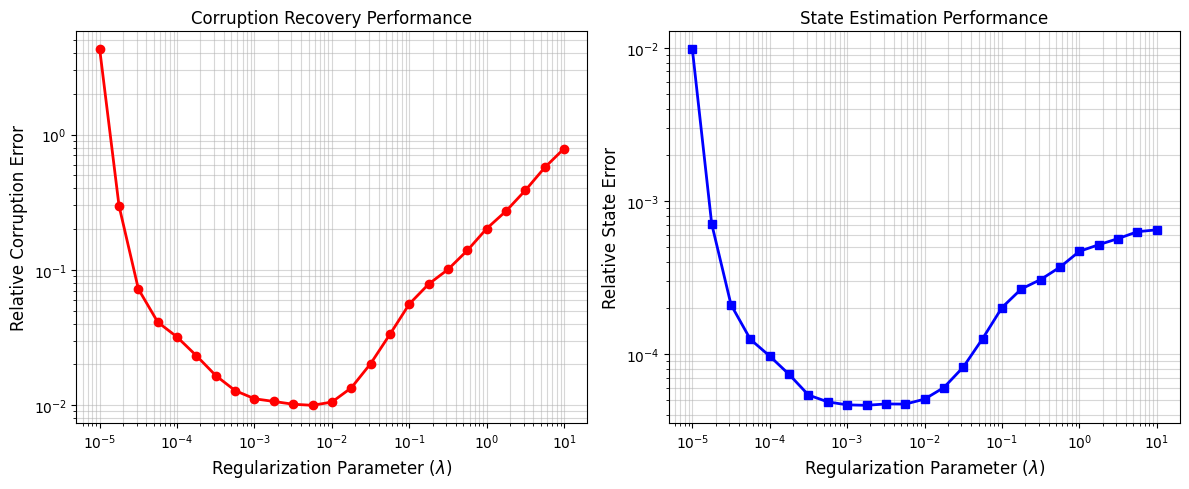
\includegraphics[width=0.9\linewidth]{recovery_error_vs_regularization.png}
    \caption{Effect of regularization on linear sparse recovery performance.}
    \label{fig:lambda_sweep_linear}
\end{figure}

\begin{figure}[t]
    \centering
    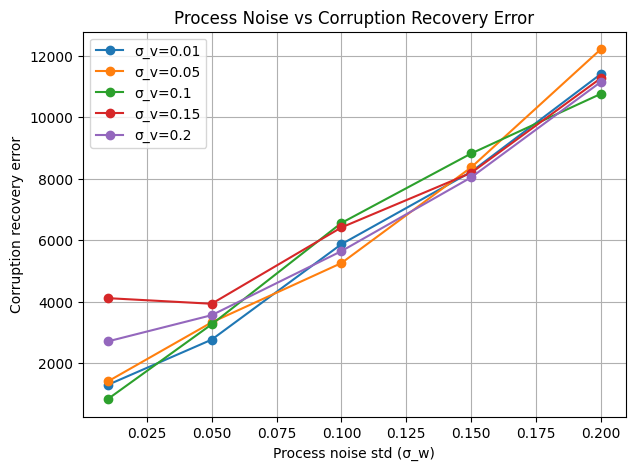
\includegraphics[width=0.9\linewidth]{process_noise_vs_recovery_error (LTI).png}
    \caption{Sensitivity of linear corruption recovery to process noise.}
    \label{fig:process_noise_linear}
\end{figure}

\begin{figure}[t]
    \centering
    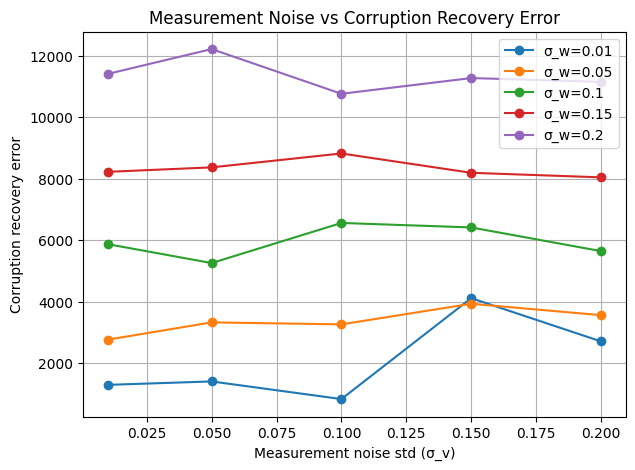
\includegraphics[width=0.9\linewidth]{measurement_noise_vs_recovery_error (LTI).png}
    \caption{Sensitivity of linear corruption recovery to measurement noise.}
    \label{fig:measurement_noise_linear}
\end{figure}

\subsection{Nonlinear Benchmark Parameters}

The nonlinear benchmark is a coupled damped pendulum chain. The state dimension is $2N$, where the first $N$ components correspond to the pendulum angles and the remaining $N$ components correspond to angular velocities. The system evolves according to the nonlinear discrete-time dynamics described in the previous section, with coupling introduced through the graph Laplacian. Sensor corruption is again injected sparsely in the measurement channels, and the output equation retains the same structure as in the linear case. \cite{nonlinearModel}


\subsection{Nonlinear Recovery Experiments}

For the nonlinear benchmark, the same regularization sweep is performed to study the dependence of bias recovery on $\lambda$. In addition, the effect of process noise and measurement noise is analyzed using relative bias recovery error. Two nonlinear solvers are compared: sequential convex programming solved via OSQP and direct nonlinear optimization solved via IPOPT. This allows the sparse recovery behavior to be evaluated under both iterative convex approximation and direct nonlinear programming. \cite{nonlinearModel}

\begin{figure}[t]
    \centering
    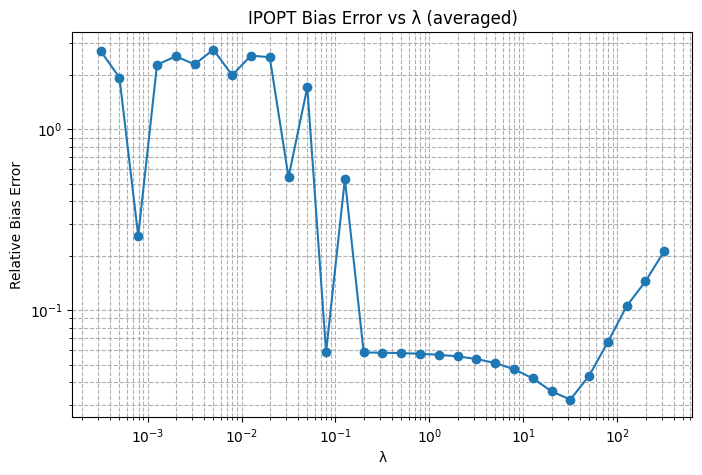
\includegraphics[width=0.9\linewidth]{IPOPT_recovery_error_vs_regularization (NL).png}
    \caption{Nonlinear sparse recovery using OSQP.}
    \label{fig:osqp_lambda}
\end{figure}

\begin{figure}[t]
    \centering
    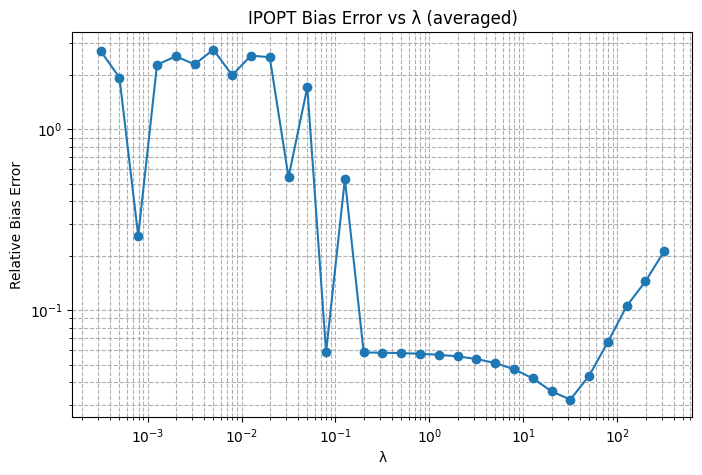
\includegraphics[width=0.9\linewidth]{IPOPT_recovery_error_vs_regularization (NL).png}
    \caption{Nonlinear sparse recovery using IPOPT.}
    \label{fig:ipopt_lambda}
\end{figure}

\begin{figure}[t]
    \centering
    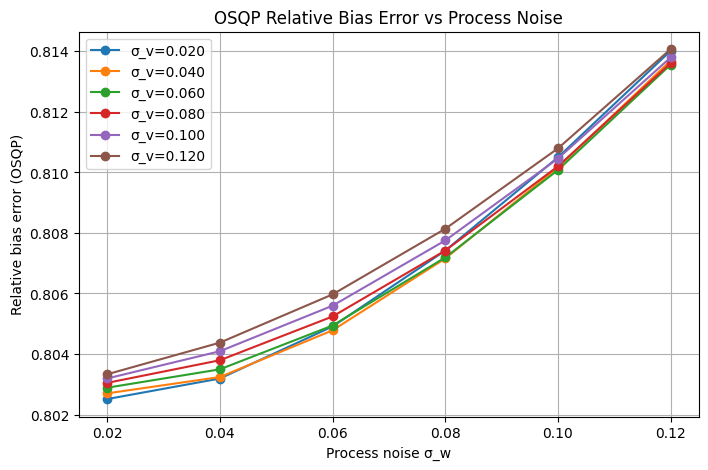
\includegraphics[width=0.9\linewidth]{OSQP_process_noise_vs_recovery_error (NL).png}
    \caption{Sensitivity of nonlinear bias recovery to process noise.}
    \label{fig:nonlinear_process_noise}
\end{figure}

\begin{figure}[t]
    \centering
    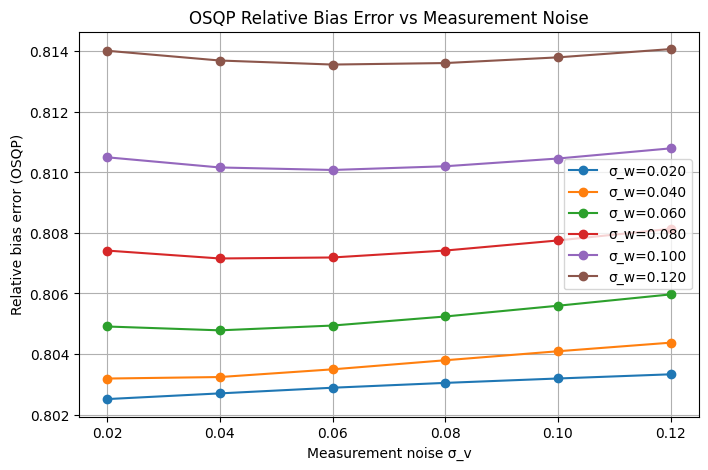
\includegraphics[width=0.9\linewidth]{OSQP_measurement_noise_vs_recovery_error (NL).png}
    \caption{Sensitivity of nonlinear bias recovery to measurement noise.}
    \label{fig:nonlinear_measurement_noise}
\end{figure}

\section{Results and Discussion}

\subsection{Linear System Results}

The linear benchmark demonstrates that sparse sensor corruption can be recovered effectively when the regularization parameter is chosen appropriately. Across the experiments, the recovery error exhibits a clear tradeoff with the sparsity weight $\lambda$. Very small values of $\lambda$ under-regularize the corruption term, while very large values suppress it excessively. As a result, the best performance is obtained at an intermediate range of $\lambda$, where the estimator balances data fidelity and sparse bias recovery. This same trend is reflected in both the corruption recovery error and the state estimation error. \cite{linearModel}

\begin{figure}[t]
    \centering
    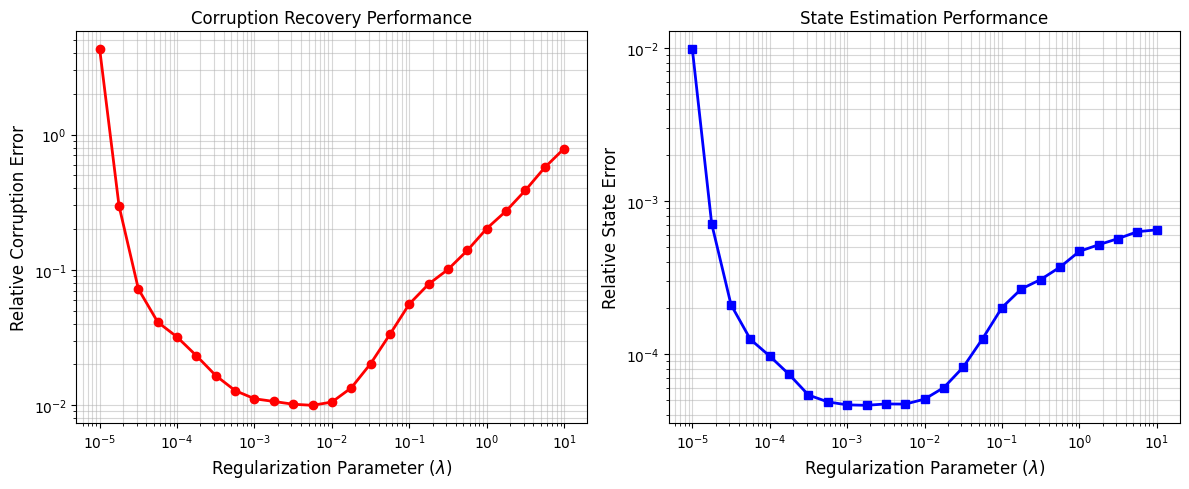
\includegraphics[width=0.9\linewidth]{recovery_error_vs_regularization.png}
    \caption{Linear system performance versus regularization parameter.}
    \label{fig:linear_results_lambda}
\end{figure}

Increasing process noise degrades the quality of sparse recovery because the state trajectory becomes harder to predict from the dynamics alone. In this regime, part of the model mismatch is absorbed into the estimated corruption term, which increases the relative recovery error. A similar effect is observed when measurement noise is increased, since noisy observations make it more difficult to distinguish true sensor bias from random perturbations. However, the trend remains stable enough to indicate that the estimator is still robust under moderate noise levels. \cite{linearModel}

\begin{figure}[t]
    \centering
    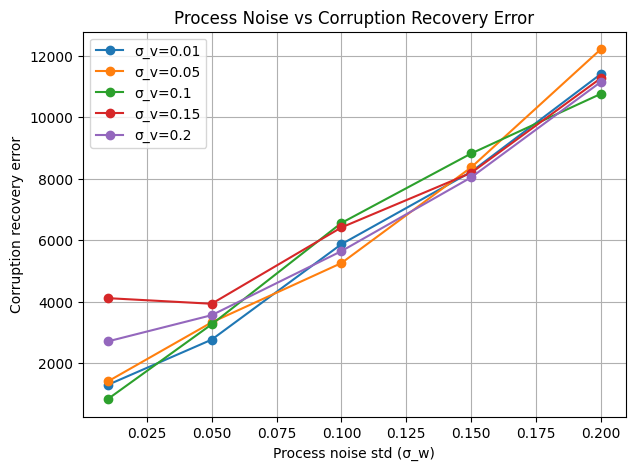
\includegraphics[width=0.9\linewidth]{process_noise_vs_recovery_error (LTI).png}
    \caption{Linear sparse recovery sensitivity to process noise.}
    \label{fig:linear_results_process_noise}
\end{figure}

\begin{figure}[t]
    \centering
    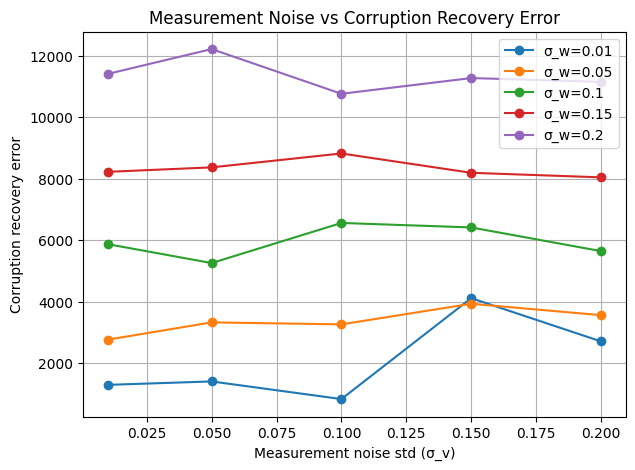
\includegraphics[width=0.9\linewidth]{measurement_noise_vs_recovery_error (LTI).png}
    \caption{Linear sparse recovery sensitivity to measurement noise.}
    \label{fig:linear_results_measurement_noise}
\end{figure}

\subsection{Nonlinear System Results}

The nonlinear pendulum benchmark shows the same fundamental sparsity tradeoff, but in a more challenging setting due to nonlinear dynamics and local coupling. Both the OSQP-based sequential convex approach and the IPOPT-based nonlinear solver show a U-shaped dependence on $\lambda$, indicating that moderate regularization again provides the best bias recovery. The agreement between the two solvers suggests that the sparse estimation behavior is not solver-specific, but rather a property of the underlying optimization structure. \cite{nonlinearModel}

% \begin{figure}[t]
%     \centering
%     \fbox{\parbox{0.9\linewidth}{\centering Placeholder for OSQP nonlinear result plot\\
%     \vspace{0.4cm}
%     Relative bias error versus $\lambda$ using OSQP.}}
%     \caption{Nonlinear sparse recovery performance using OSQP.}
%     \label{fig:nonlinear_results_osqp}
% \end{figure}

% \begin{figure}[t]
%     \centering
%     \fbox{\parbox{0.9\linewidth}{\centering Placeholder for IPOPT nonlinear result plot\\
%     \vspace{0.4cm}
%     Relative bias error versus $\lambda$ using IPOPT.}}
%     \caption{Nonlinear sparse recovery performance using IPOPT.}
%     \label{fig:nonlinear_results_ipopt}
% \end{figure}

The process noise and measurement noise studies confirm that larger disturbances make sparse bias recovery more difficult, although the degradation is gradual in the tested regime. This indicates that the estimator remains numerically stable while still being sensitive to the expected sources of uncertainty. The Laplacian coupling in the pendulum chain also makes the problem more realistic, since local disturbances propagate across neighboring states and increase the difficulty of isolating sensor corruption. \cite{nonlinearModel}

% \begin{figure}[t]
%     \centering
%     \fbox{\parbox{0.9\linewidth}{\centering Placeholder for nonlinear process noise result plot\\
%     \vspace{0.4cm}
%     Relative bias error versus process noise.}}
%     \caption{Nonlinear sparse recovery sensitivity to process noise.}
%     \label{fig:nonlinear_results_process_noise}
% \end{figure}

% \begin{figure}[t]
%     \centering
%     \fbox{\parbox{0.9\linewidth}{\centering Placeholder for nonlinear measurement noise result plot\\
%     \vspace{0.4cm}
%     Relative bias error versus measurement noise.}}
%     \caption{Nonlinear sparse recovery sensitivity to measurement noise.}
%     \label{fig:nonlinear_results_measurement_noise}
% \end{figure}

\subsection{Discussion}

Across both benchmarks, the experiments show a consistent pattern: sparse corruption can be recovered well when the regularization is balanced, but performance degrades as process noise and measurement noise increase. The linear case demonstrates the basic effectiveness of the $L_1$ relaxation, while the nonlinear pendulum network shows that the same approach extends to more realistic dynamics when combined with sequential convex programming or nonlinear optimization. Overall, the results support the use of sparse regularization as a practical tool for robust state estimation under corrupted sensing. \cite{linearModel,nonlinearModel}


\section{Conclusion}

This project investigated sparse state estimation under sensor corruption for both linear and nonlinear dynamical systems. The estimation framework combined batch optimization with sparse regularization in order to jointly recover the hidden system states and identify corrupted sensor measurements. By modeling sensor corruption as a sparse additive bias, the estimation problem was formulated as an optimization problem with an $L_1$ regularization term that promotes sparsity while remaining computationally tractable.

For the linear benchmark, the proposed estimator successfully recovered sparse sensor corruption under partial observation and noisy measurements. The experiments demonstrated that the choice of regularization parameter plays a critical role in balancing sparsity and data fidelity. Moderate regularization consistently produced the best corruption recovery and state estimation performance, while excessive process noise and measurement noise reduced estimation accuracy by increasing ambiguity between stochastic disturbances and sparse corruption.

The nonlinear pendulum benchmark extended the same sparse recovery framework to a coupled nonlinear system with Laplacian interaction between neighboring states. Sequential convex programming using OSQP and direct nonlinear optimization using IPOPT both produced stable recovery trends and showed similar dependence on the regularization parameter. Although the nonlinear setting introduced additional complexity due to nonlinear coupling and local interactions, the sparse optimization framework remained effective for recovering corrupted measurements.

Overall, the results demonstrate that sparse optimization techniques provide a practical and robust approach for state estimation in corrupted sensing environments. The framework developed in this work can be extended further toward online moving-horizon estimation, adversarial attack detection, distributed estimation for networked systems, and robust estimation for higher-dimensional nonlinear robotic systems.
\bibliographystyle{IEEEtran}
\bibliography{refs}

\end{document}
